\chapter{Sprint 4 -- LLM Integration and Realistic Data Enrichment}

\setlength{\textfloatsep}{8pt plus 2pt minus 2pt}
\setlength{\floatsep}{8pt plus 2pt minus 2pt}
\setlength{\intextsep}{8pt plus 2pt minus 2pt}
\setlength{\abovecaptionskip}{4pt}
\setlength{\belowcaptionskip}{0pt}

\section*{Introduction}
\addcontentsline{toc}{section}{Introduction}

\paragraph{}QA engineers need test data that is not only valid, but also easy to read and recognize.
Realistic labels and descriptions make generated records clearer in Longview screens, logs, and
validation results, which helps identify functional errors faster.

\paragraph{}For this reason, Sprint 4 keeps the generator pipeline from the previous sprints, then adds
an optional Large Language Model enrichment step after base generation and before validation. The LLM
does not decide the structure of the dataset. It only improves readable fields such as names,
symbols, descriptions, account labels, group labels, and model labels.

\section{Sprint Backlog}

\paragraph{}The sprint backlog was therefore focused on one objective: make generated data more
realistic without weakening the deterministic generation rules. Table~\ref{tab:sprint4-backlog}
summarizes the planned work.

\small
\renewcommand{\arraystretch}{1.05}
\begin{longtable}{|Q{0.07\linewidth}|P{0.29\linewidth}|P{0.42\linewidth}|Q{0.12\linewidth}|}
\caption{Sprint 4 backlog}
\label{tab:sprint4-backlog} \\
\hline
\textbf{ID} & \textbf{Task} & \textbf{Description} & \textbf{Estimate} \\
\hline
\endfirsthead
\multicolumn{4}{r}{\tablename\ \thetable{} -- \textit{continued from previous page}} \\
\hline
\textbf{ID} & \textbf{Task} & \textbf{Description} & \textbf{Estimate} \\
\hline
\endhead
\hline
\multicolumn{4}{r}{\textit{continued on next page}} \\
\endfoot
\hline
\endlastfoot
T4-1 & Add LLM module & Integrate the LLM client, service layer, prompt files, and enrichers into the NestJS backend. & 2 days \\
\hline
T4-2 & Define enrichable fields & Identify which fields may be modified for securities, accounts, account groups, and models. & 1 day \\
\hline
T4-3 & Write controlled prompts & Build prompts that request structured values and avoid changing relationships or numeric data. & 2 days \\
\hline
T4-4 & Implement enrichment services & Apply enrichers for securities, accounts, account groups, and models after base generation. & 3 days \\
\hline
T4-5 & Add fallback behavior & Preserve deterministic values when enrichment is disabled, unavailable, malformed, or incomplete. & 2 days \\
\hline
T4-6 & Validate enriched output & Run the same generator validation after enrichment and before SQL script assembly. & 1 day \\
\hline
\end{longtable}
\normalsize
\renewcommand{\arraystretch}{1}

\section{Sprint Specification}

\paragraph{}From the QA engineer's point of view, the workflow remains the same: select the data,
configure the generation, preview if needed, and launch the output. The enrichment decision is
handled internally by the backend according to provider availability, response validity, and dataset
size.

\subsection{Functional Requirements}

\paragraph{}Table~\ref{tab:sprint4-functional-requirements} lists the functional requirements. Numerical
and structural data remain generated by deterministic algorithms.

\renewcommand{\arraystretch}{1.15}
\begin{longtable}{|P{0.27\linewidth}|P{0.23\linewidth}|P{0.40\linewidth}|}
\caption{Functional requirements of Sprint 4}
\label{tab:sprint4-functional-requirements} \\
\hline
\textbf{Requirement} & \textbf{Responsible component} & \textbf{Description} \\
\hline
\endfirsthead
\multicolumn{3}{r}{\tablename\ \thetable{} -- \textit{continued from previous page}} \\
\hline
\textbf{Requirement} & \textbf{Responsible component} & \textbf{Description} \\
\hline
\endhead
\hline
\multicolumn{3}{r}{\textit{continued on next page}} \\
\endfoot
\hline
\endlastfoot
Configure generation request & QA engineer & Select the data to generate and define the generation parameters. \\
\hline
Generate test data & QA engineer & Launch standalone or connected generation from the selected configuration. \\
\hline
Check LLM availability & Generation service & Decide whether the LLM enrichment layer can be used for the current request. \\
\hline
Enrich supported descriptive fields & LLM enrichment module & Improve securities, accounts, account groups, and portfolio model labels or descriptions. \\
\hline
Validate enriched data & Generation service & Ensure that enriched values still respect field constraints and generation rules. \\
\hline
Use algorithmic fallback & Generation service & Keep deterministic values when LLM enrichment is disabled, unavailable, invalid, or unsuitable for a large-volume request. \\
\hline
\end{longtable}
\renewcommand{\arraystretch}{1}

\subsection{Internal Enrichment Scenario}

\renewcommand{\arraystretch}{1.12}
\begin{longtable}{|P{0.24\linewidth}|P{0.66\linewidth}|}
\caption{Textual description of the internal LLM enrichment scenario}
\label{tab:llm-usecase-description} \\
\hline
\textbf{Element} & \textbf{Description} \\
\hline
\endfirsthead
\multicolumn{2}{r}{\tablename\ \thetable{} -- \textit{continued from previous page}} \\
\hline
\textbf{Element} & \textbf{Description} \\
\hline
\endhead
\hline
\multicolumn{2}{r}{\textit{continued on next page}} \\
\endfoot
\hline
\endlastfoot
Use case & Enrich generated data with realistic descriptive values. \\
\hline
Actor & Backend generation service, triggered by the QA Engineer's generation request. \\
\hline
Preconditions &
\begin{itemize}[leftmargin=*,nosep]
    \item A valid standalone or connected generation request was launched.
    \item Base data was generated successfully.
    \item LLM enrichment is enabled and at least one Gemini API key is available.
    \item The section stays within safe limits: 5,000 securities, 1,000 accounts, 1,000 account groups, or 1,000 model rows.
\end{itemize} \\
\hline
Postconditions & Valid enriched values are merged into the generated dataset and reported in logs.
If enrichment is skipped or unsafe, deterministic values remain valid and generation continues. \\
\hline
Main scenario &
\begin{enumerate}[leftmargin=*,nosep]
    \item The pipeline creates the deterministic dataset.
    \item \texttt{LlmService} receives securities, models, accounts, and groups.
    \item It checks availability and section size limits.
    \item The proper enricher builds the prompt; securities are chunked by kind.
    \item Gemini is called through the model/key fallback route.
    \item JSON is checked for count, IDs, and security kinds.
    \item Only readable fields are merged: names, labels, descriptions, symbols, or issuer labels.
    \item Final validation and output assembly.
\end{enumerate} \\
\hline
Enrichment rules &
\begin{itemize}[leftmargin=*,nosep]
    \item Enrichment applies only to securities, accounts, account groups, and models.
    \item Numbers, dates, prices, quantities, allocations, relationship identifiers, and loading order stay algorithmic.
    \item Prompts enforce JSON-only output, expected object count, business context, and field-length constraints.
    \item The client queues requests, limits concurrency, and tries Gemini Flash before Flash Lite with the configured keys.
\end{itemize} \\
\hline
Exception scenario &
\begin{itemize}[leftmargin=*,nosep]
    \item If LLM is disabled, missing, unreachable, timed out, rate-limited, or denied, the system uses the fallback algorithms.
    \item If a section is larger than the safe enrichment limit, enrichment is skipped for that section and the system uses the fallback algorithms.
    \item If the response is empty, malformed, truncated, wrong-count, wrong-ID, or wrong-kind, the system uses the fallback algorithms.
    \item If final validation fails, SQL output is blocked until the generated data is corrected.
\end{itemize} \\
\hline
\end{longtable}
\renewcommand{\arraystretch}{1}

\section{Sprint Design}

\paragraph{}The design isolates the LLM behind dedicated client and enricher classes so that the
generation services remain responsible for data structure, validation, and SQL output.

\subsection{Sequence Diagrams}

\paragraph{}Figure~\ref{fig:sequence-llm} shows the enrichment sequence and fallback branch.

\begin{figure}[!htbp]
\centering
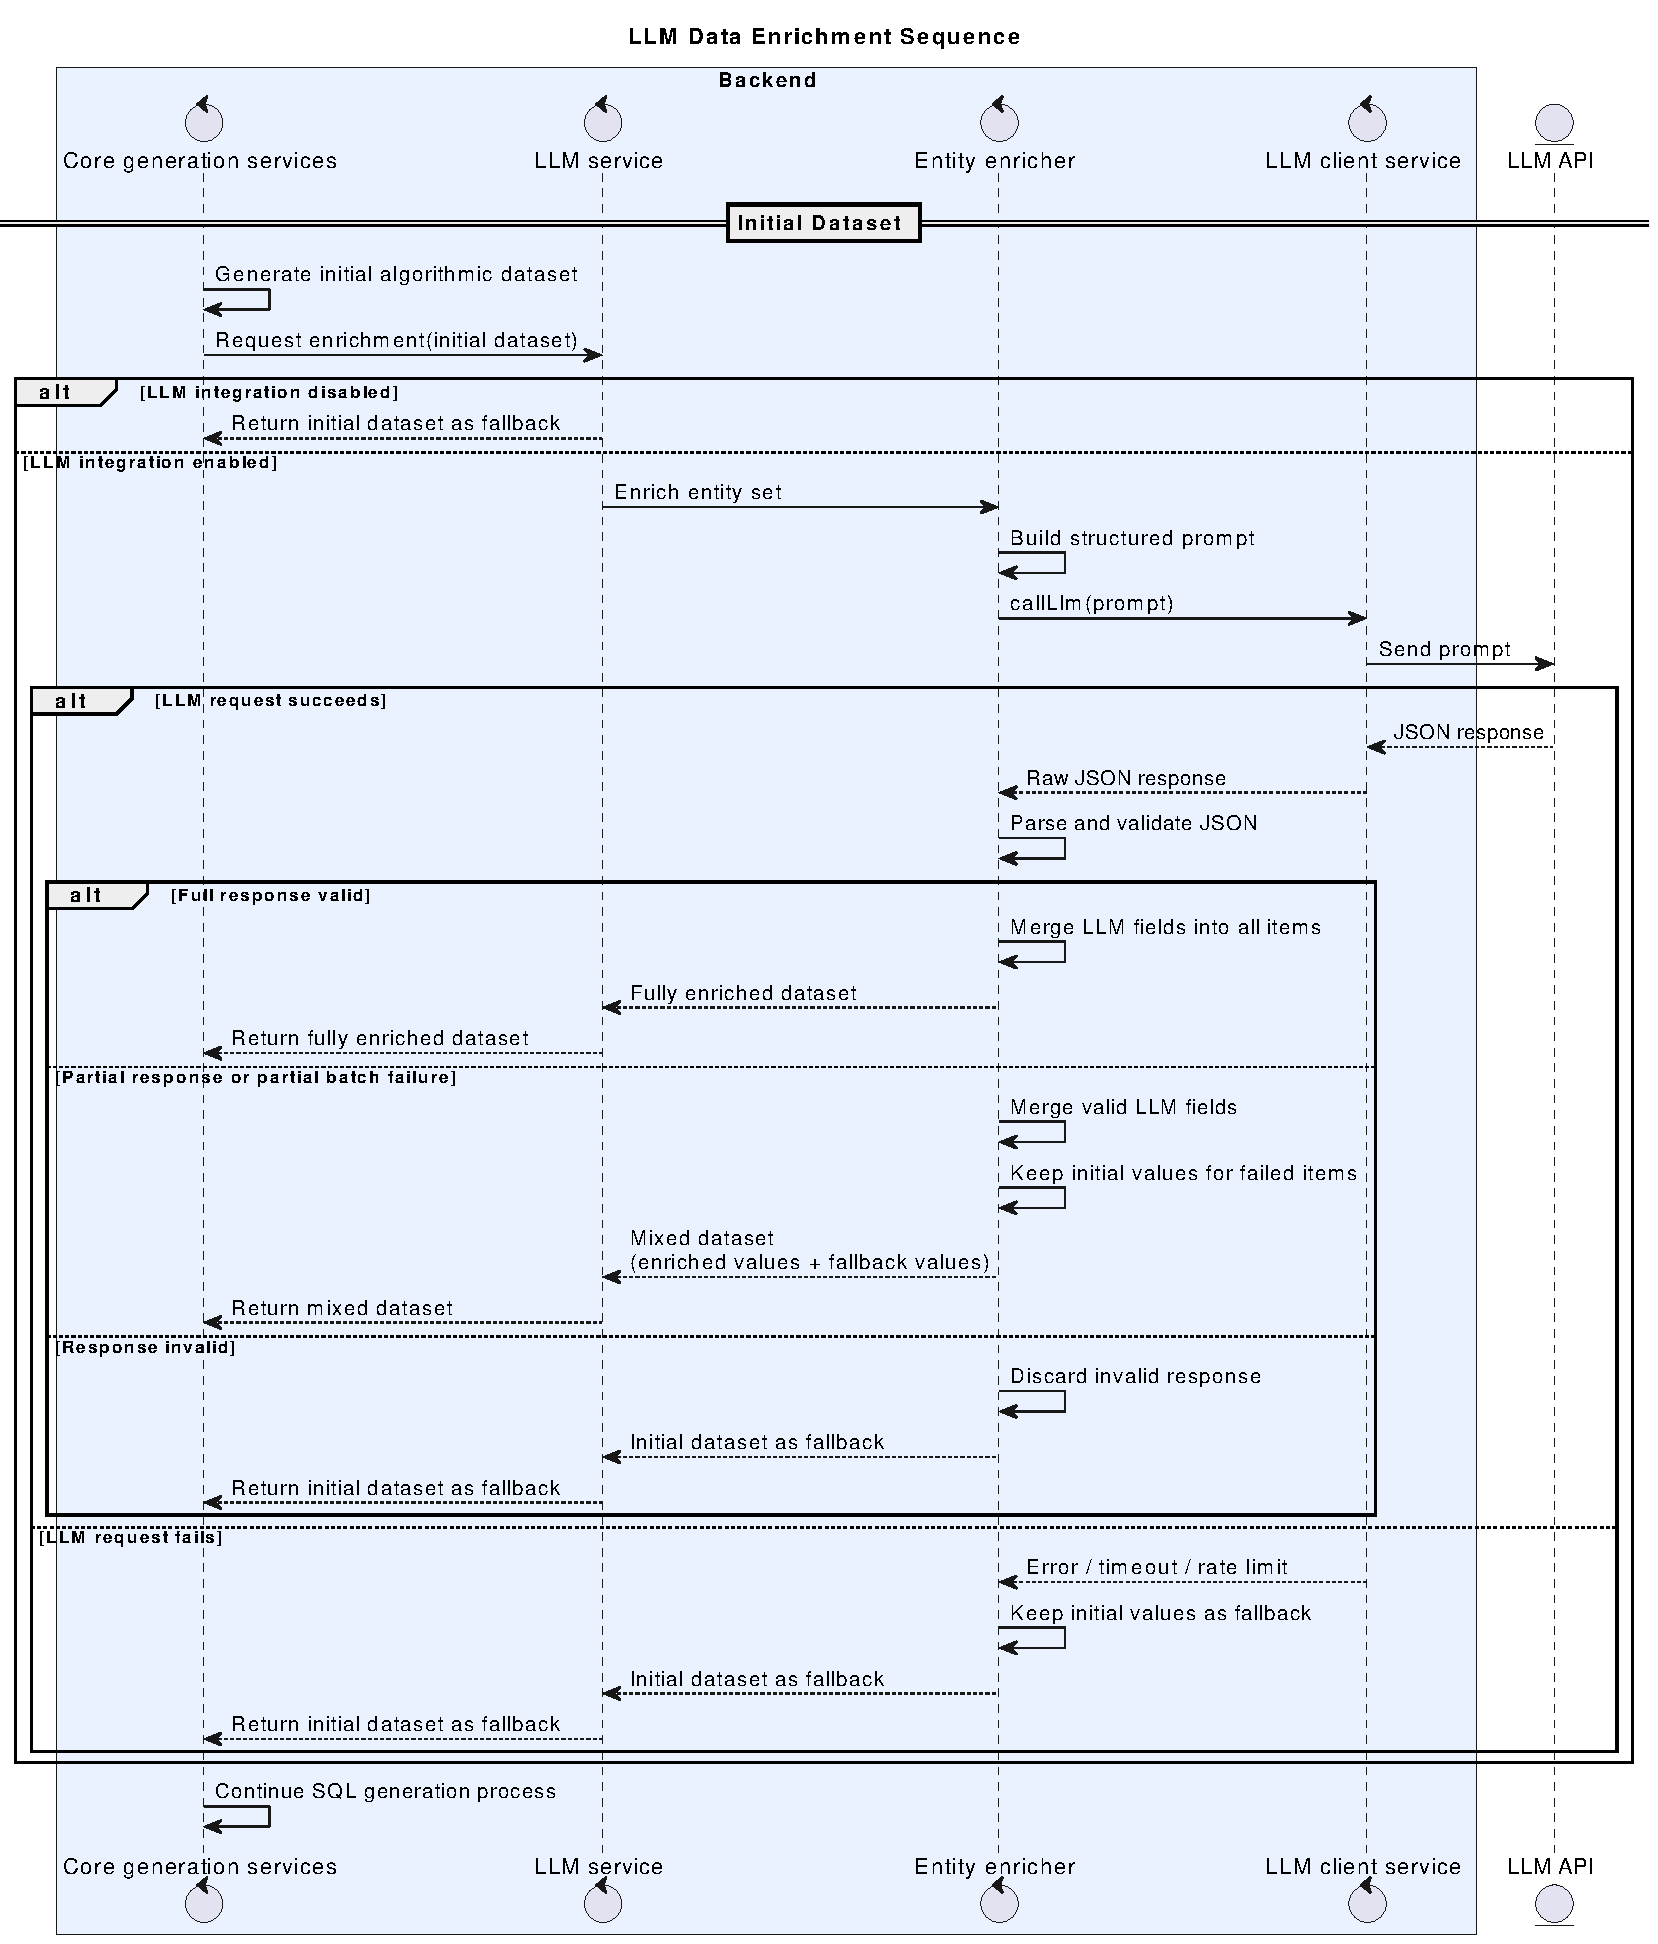
\includegraphics[width=0.95\textwidth]{img/sequence-llm-enrichment.pdf}
\caption{LLM enrichment sequence}
\label{fig:sequence-llm}
\end{figure}

\subsection{Class Diagram of Sprint 4}

\paragraph{}Figure~\ref{fig:sprint4-class-diagram} presents the main enrichment classes.

\begin{figure}[!htbp]
\centering
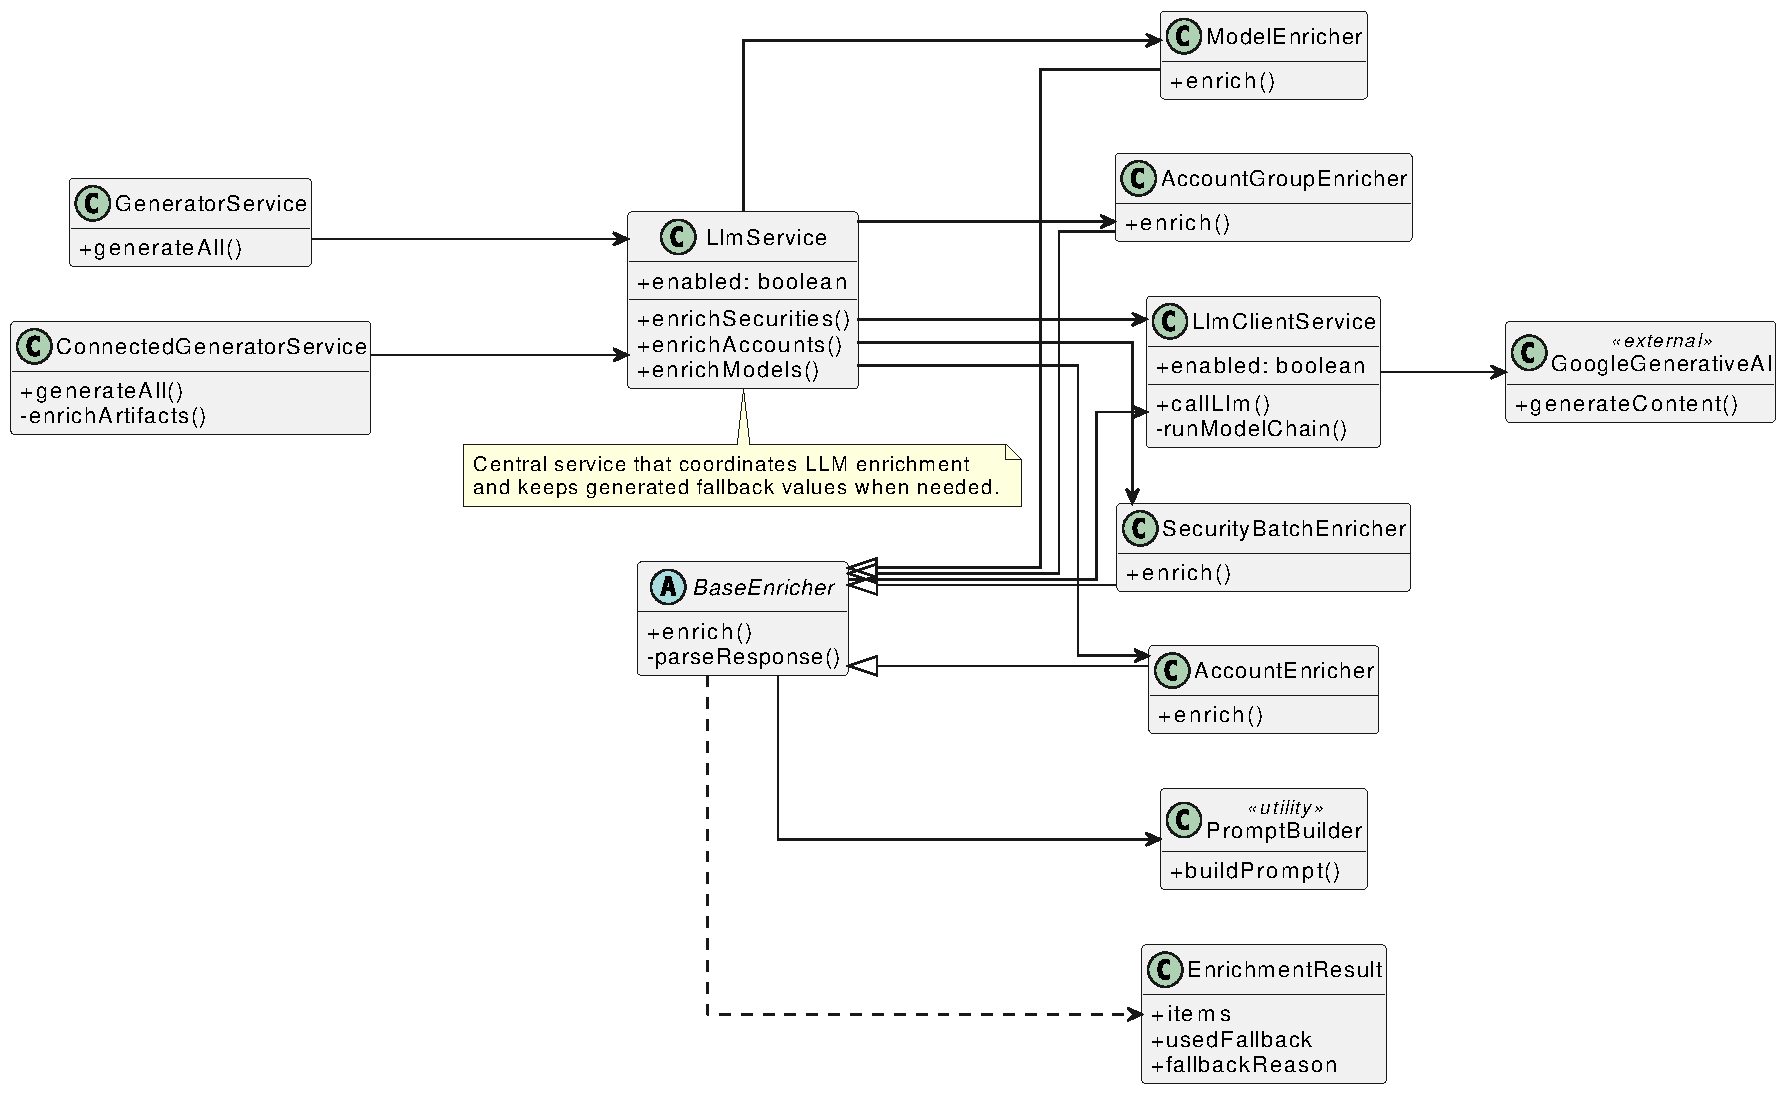
\includegraphics[width=0.95\textwidth]{img/llm-class-diagram.pdf}
\caption{Class diagram of Sprint 4}
\label{fig:sprint4-class-diagram}
\end{figure}

\subsection{LLM Provider Choice}

\paragraph{}Gemini was selected for this sprint because it offered a practical free-tier option during
development and provided enough quality for short financial text enrichment tasks. The objective was
not advanced reasoning, but fast generation of structured labels, symbols, and descriptions. For that
reason, the implementation uses Gemini 2.5 Flash as the preferred model and Gemini 2.5 Flash Lite as
the lighter fallback route before returning to algorithmic values.

\subsection{Prompt Engineering Strategy}

\paragraph{}Because the LLM receives only a controlled enrichment task, prompt engineering is centered
on structure and safety rather than open-ended generation. Table~\ref{tab:prompt-engineering-rules}
summarizes the rules used by the dedicated prompt builders.

\Needspace{11\baselineskip}
\renewcommand{\arraystretch}{1.25}
\begin{longtable}{|P{0.26\linewidth}|P{0.64\linewidth}|}
\caption{Prompt engineering rules used in Sprint 4}
\label{tab:prompt-engineering-rules} \\
\hline
\textbf{Rule} & \textbf{Implementation in the project} \\
\hline
\endfirsthead
\multicolumn{2}{r}{\tablename\ \thetable{} -- \textit{continued from previous page}} \\
\hline
\textbf{Rule} & \textbf{Implementation in the project} \\
\hline
\endhead
\hline
\multicolumn{2}{r}{\textit{continued on next page}} \\
\endfoot
\hline
\endlastfoot
Domain-specific prompts & Separate prompts are used for securities, accounts, account groups, and models. This avoids mixing unrelated instructions. \\
\hline
Business context & Prompts include useful context such as reference date, currencies, and the type of financial object to enrich. \\
\hline
JSON-only response & The LLM is instructed to return only a valid JSON array, without markdown, comments, explanations, or code fences. \\
\hline
Exact quantity control & The requested number of objects must match the number of objects returned by the LLM. If the count is wrong, fallback is used. \\
\hline
Identifier preservation & The LLM must copy backend-provided identifiers. This allows the enrichers to map each response to the correct generated record. \\
\hline
Allowed fields only & Each prompt lists only the fields that may be enriched, such as labels, names, symbols, or descriptions. Structural fields are never delegated to the LLM. \\
\hline
Response validation & The backend parses the JSON, checks expected IDs and types, applies maximum field lengths, and keeps deterministic values when the response is invalid. \\
\hline
\end{longtable}
\renewcommand{\arraystretch}{1}

\section{Realization}

\paragraph{}The backend implementation is located in \texttt{modules/llm}. Both standalone and connected
generation call \texttt{LlmService} after base records are created, then continue through the same
validation and output assembly steps used in the previous sprints.

\subsection{Internal Generation and LLM Enrichment Comparison}

\paragraph{}Table~\ref{tab:internal-vs-llm-comparison} shows why the LLM layer improves the
generator for QA work while the internal algorithm remains necessary for structure, volume, and
fallback.

\Needspace{13\baselineskip}
\renewcommand{\arraystretch}{1.3}
\begin{longtable}{|P{0.22\linewidth}|P{0.30\linewidth}|P{0.30\linewidth}|}
\caption{Comparison between internal generation and LLM-assisted enrichment}
\label{tab:internal-vs-llm-comparison} \\
\hline
\textbf{Criterion} & \textbf{Internal algorithm generation} & \textbf{LLM-assisted enrichment} \\
\hline
\endfirsthead
\multicolumn{3}{r}{\tablename\ \thetable{} -- \textit{continued from previous page}} \\
\hline
\textbf{Criterion} & \textbf{Internal algorithm generation} & \textbf{LLM-assisted enrichment} \\
\hline
\endhead
\hline
\multicolumn{3}{r}{\textit{continued on next page}} \\
\endfoot
\hline
\endlastfoot
Generation role & Produces valid rows, relationships, and loading order. & Improves only the readable fields after the valid dataset already exists. \\
\hline
Readability for QA & Technically valid, but names and labels can be generic or repetitive. & Produces clearer business-like names, labels, symbols, and descriptions. \\
\hline
Error detection & Harder to inspect in Longview when many records look similar. & Easier to recognize abnormal data because generated values look closer to real financial data. \\
\hline
Domain coherence & Applies fixed rules without understanding the business meaning of text fields. & Uses prompt context such as currencies, dates, entity type, and field constraints to create more coherent text. \\
\hline
Large data volumes & Best option for bulk generation and performance tests. & Used selectively because realistic enrichment is more useful for readable test sets than huge volume tests. \\
\hline
Safety & Deterministic and reproducible. & Safe because it cannot change IDs, quantities, prices, dates, relationships, or loading rules. \\
\hline
Final value & Guarantees that generation still works without external services. & Adds realism where it matters, with automatic fallback to the internal algorithm. \\
\hline
\end{longtable}
\renewcommand{\arraystretch}{1}

\subsection{API Key and Model Fallback Strategy}

\paragraph{}Figure~\ref{fig:llm-availability-fallback} shows the route used by the enrichment client. The
system first tries the two configured API keys with the preferred Gemini model, then with the lighter
fallback model. If no route returns a valid JSON response, deterministic values are kept.

\begin{figure}[!htbp]
\centering
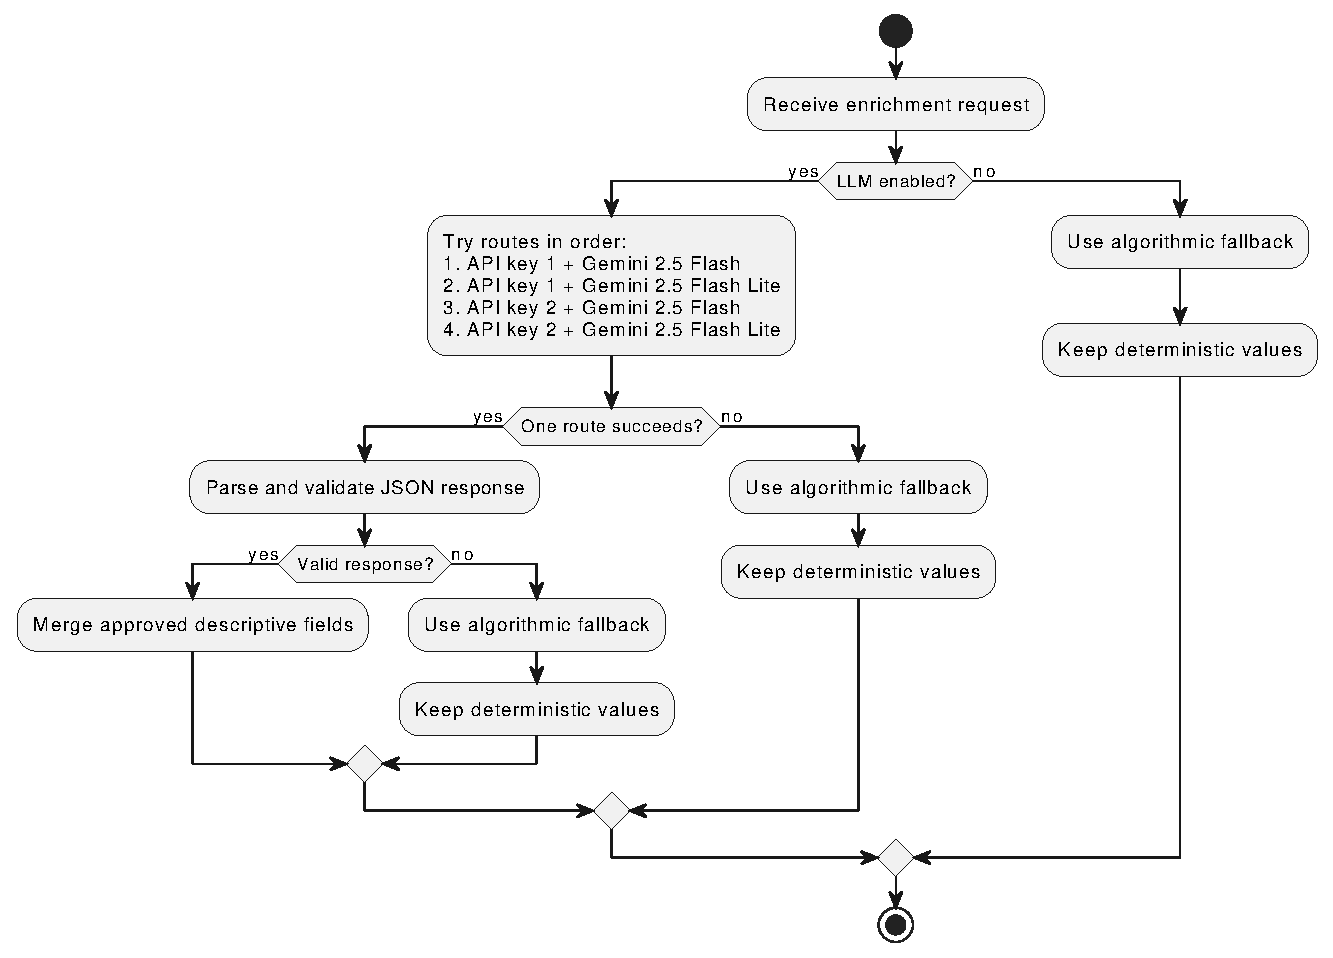
\includegraphics[width=0.82\textwidth]{img/llm-availability-fallback.pdf}
\caption{LLM availability and fallback mechanism}
\label{fig:llm-availability-fallback}
\end{figure}

\subsection{Implemented Components}

\renewcommand{\arraystretch}{1.15}
\begin{longtable}{|P{0.24\linewidth}|P{0.34\linewidth}|P{0.32\linewidth}|}
\caption{Main implemented LLM components}
\label{tab:llm-realization} \\
\hline
\textbf{Realized element} & \textbf{Project source} & \textbf{Role} \\
\hline
\endfirsthead
\multicolumn{3}{r}{\tablename\ \thetable{} -- \textit{continued from previous page}} \\
\hline
\textbf{Realized element} & \textbf{Project source} & \textbf{Role} \\
\hline
\endhead
\hline
\multicolumn{3}{r}{\textit{continued on next page}} \\
\endfoot
\hline
\endlastfoot
LLM facade & \texttt{llm.service.ts} & Coordinates enrichment for securities, accounts, groups, and models. \\
\hline
Provider client & \texttt{llm-client.service.ts} & Calls the AI provider and handles availability or parsing failures. \\
\hline
Security enrichment & \texttt{security-batch.enricher.ts} & Enriches multiple security subtypes with controlled textual values. \\
\hline
Account and group enrichment & \texttt{account.enricher.ts}, \texttt{account-group.enricher.ts} & Improves account labels while preserving account structure. \\
\hline
Model enrichment & \texttt{model.enricher.ts} & Improves model labels without changing allocation relationships. \\
\hline
Fallback behavior & \texttt{fallback-reason.util.ts} & Explains why deterministic values were kept when enrichment is unsafe. \\
\hline
\end{longtable}
\renewcommand{\arraystretch}{1}

\paragraph{}Figure~\ref{fig:ch6-llm-proof} is reserved as the realization proof for this sprint. It
should show an enriched generation result, a fallback log, or a before/after comparison of readable
fields produced by the LLM layer.

\begin{figure}[!htbp]
\centering
\IfFileExists{img/ch6-llm-proof.png}{%
    \includegraphics[width=0.88\textwidth]{img/ch6-llm-proof.png}%
}{%
    \fbox{\parbox[c][0.22\textheight][c]{0.86\textwidth}{\centering Screenshot to be added: LLM enrichment result, fallback log, or before/after enriched data comparison}}%
}
\caption{LLM enrichment output and fallback evidence}
\label{fig:ch6-llm-proof}
\end{figure}

\section*{Conclusion}
\addcontentsline{toc}{section}{Conclusion}

\paragraph{}Sprint 4 delivered controlled LLM enrichment for readable financial fields while preserving
the deterministic generation pipeline. The application can now improve labels, names, symbols, and
descriptions when the LLM is available, and keep algorithmic values when enrichment is unsafe,
unavailable, or unsuitable for large-volume tests.
